\documentclass[a4paper]{article}

\usepackage{listings}
\usepackage{graphicx}
\usepackage{fancyhdr}
\usepackage{color}
\usepackage{xcolor}
\pagestyle{fancy}

\lhead{Tube Tracker}
\rhead{CSN08113}
\lfoot{Final Report}
\cfoot{\thepage}
\rfoot{Gareth Pulham, 40099603}

\lstdefinestyle{customc}{
    belowcaptionskip=1\baselineskip,
    frame=single,
    xleftmargin=\parindent,
    language=C,
    showstringspaces=false,
    basicstyle=\footnotesize\ttfamily,
    keywordstyle=\bfseries\color{green!40!black},
    commentstyle=\itshape\color{purple!40!black},
    identifierstyle=\color{blue},
    stringstyle=\color{orange},
}


\begin{document}
    \begin{titlepage}
        \title{Physical Computing CSN08113\\
            Tube Tracker
        }
        \author{Gareth Pulham, 40099603}
        \date{\today}
        \maketitle
        \thispagestyle{empty}

        \begin{abstract}
            This project aims to produce a “Tube Tracker”, a device which can be used to identify the location of a catheter inside the body by detecting the metal guide wire when placing it.
            To do so, the device interprets signals produced by a COTS metal detector commonly used for security purposes.

            By examining and measuring the metal detectors internal construction, it was possible to identify and interpret the strength of metal detection, which can then be displayed to the user to deduce the location of the guide wire.

            As a result of this work, a working prototype was developed and demonstrated.

            This project was undertaken in partnership with Megan Currie, a product design student at Edinburgh Napier University, who developed the concept and packaging for this project.
        \end{abstract}
    \end{titlepage}

    \tableofcontents

    \section{Introduction}
    Blah blah blah, this is the introduction.

    \section{Post-Introduction}
    Lorem  ipsum  dolor  sit  amet,  consectetuer  adipiscing  
    elit.   Etiam  lobortisfacilisis sem.  Nullam nec mi et 
    neque pharetra sollicitudin.  Praesent imperdietmi nec ante. 
    Donec ullamcorper, felis non sodales...

    \section{Schematic}
    \begin{figure}[h]
        \centering
        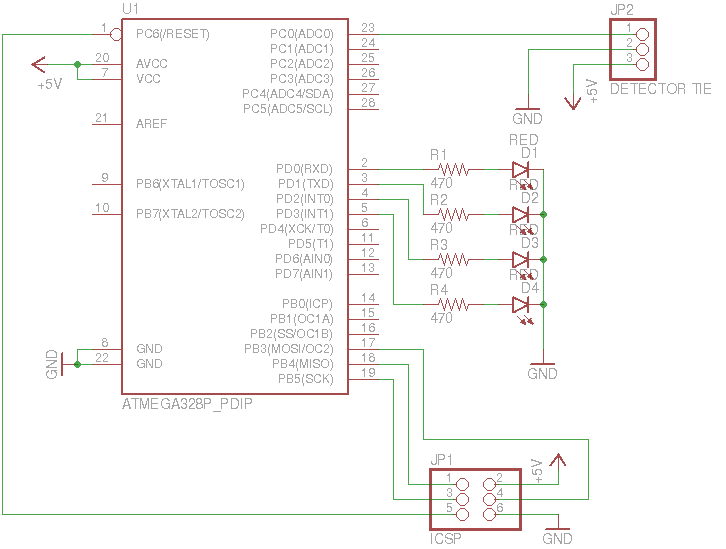
\includegraphics[width=0.75\textwidth]{images/schematic}
        \caption{It's the schematics}
    \end{figure}


    \section{Source}
    \lstinputlisting[style=customc]{../src/tracker.c}

\end{document}
